\subsection{ \og Stigmergie \fg{} }

À fin de bien séparer la logique liée à la réflexion de celle qui structure le jeu, nous suivrons le paradigme \og Agent et Environnement \fg{}. Notre intelligence artificielle sera assimilée à un agent qui évolue dans un environnement qu'il peut observer et modifier. 
Toute communication entre agents se fera donc par \og Tableau Noir \fg{}, c'est à dire en laissant des traces dans cet environnement partagé. Cette interaction dite \og Stigmergique \fg{} est nécessairement asynchrone mais possède l'avantage de ne nécessiter qu'un seul canal de communication par agent.
Ce canal, reliant l'agent à son environnement, est bidirectionnelle: il permettra à l'agent de recevoir des stimuli et d'envoyer des impulsions. Par la suite nous parlerons de \og percepts\fg{} et \og actions\fg{}:

\begin{figure}[H] 
\centering
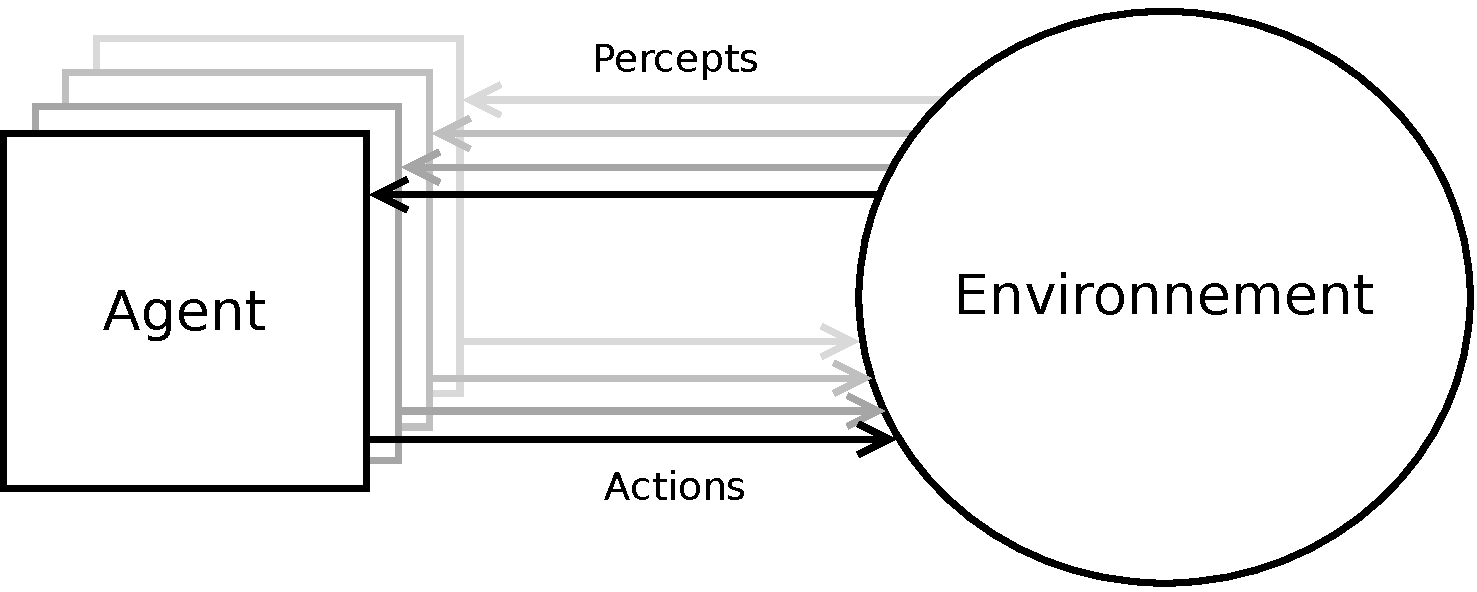
\includegraphics[width=\textwidth]{files/env/agent_env} 
\caption{Schéma du modèle \og Agent et Environnement \fg{}} 
\label{agent_env}
\end{figure}

En séparant l'agent de son environnement nous avons gagnés beaucoup de flexibilité: l'agent peut être aussi bien un humain qu'une machine. Celle-ci pouvant être notre système aussi bien qu'une intelligence artificielle tiers. 
En effet, tant que celui-ci n'a besoin de pouvoir communiquer avec son environnement qu'à travers des envoies de messages précises, tout algorithme pourrait être encapsulé avec une interface simple pour en faire un agent. Nous nous abstrairions ainsi du fonctionnement interne de chaque agent.
Cette abstraction permettra d'une part d'évaluer notre agent à la fin du développement, en le faisant joueur contre un autre agent basé sur une stratégie connu. D'autre part nous pourrions tester échafaudage de l'application en cours d'implémentation sans que nous ayons besoin pour autant que notre propre agent soit encore fonctionnelle. Le développement de la plateforme de teste sera alors complètement découplé de celui de l'IA.

\subsection{ Agent \og Arbitre \fg{} }

Dans notre cas l'environnement est un jeu de plateau, donc une grille dont les cases peuvent contenir un pion ou être vide. L'environnement doit aussi "connaître", pour ainsi dire, quel est le prochain joueur qui doit jouer ainsi que toute autre information qui ne peut pas être directement déduite de l'état du plateau. Finalement il doit pouvoir juger de la légalité des coups proposés par l'agent, et par le même biais savoir comment initialiser le plateau de la bonne manière.
Il se décompose donc en trois modules: un plateau, une liste de règles et un processeur qui les manipule. Au lieu de briser le métaphore du \og Tableau Noir \fg{} en parlant d'environnement-agent, nous ce processeur sera en effet un agent tiers: une sorte d'arbitre neutre. C'est un agent purement réactif qui maintient l'état du jeu en exécutant les coups qui lui sont envoyés par les agents joueurs dans la mesure du légale. Il devrait bien-sur les notifier de l'éventuelle faillite de leurs actions, ainsi que leur envoyer l'état du plateau en cas de demande. 

%    ---------- ACTION --------->              PROCESSEUR                ---------- RESULTAT --------->
%                                       /                      \
%                             consulte /                        \ pour modifier
%                                     v                          v
%                                    RÈGLES                  PLATEAU

Finalement c'est à travers cet agent-filtre que les autres iront modifier l'environnement et donc communiquer entre eux. Suite à cette étude préalable, il nous semble claire qu'une architecture client-serveur serait recommandé pour l'implémentation des interactions entre les agents et leur environnement.